\documentclass[a4paper,14pt]{extarticle}
\usepackage{../../tex-shared/report-layout}

\renewcommand{\mylabnumber}{5}
\renewcommand{\mylabtitle}{Исследование моделей взаимодействия распределенно выполняющихся процессов}
\renewcommand{\mysubject}{Теория распределенных систем и параллельных вычислений}
\renewcommand{\mylecturer}{Дрозин А.Ю.}

\begin{document}
\begin{titlepage}
    
    \thispagestyle{empty}
    
    \begin{center}
        
        Министерство науки и Высшего образования Российской Федерации \\
        Севастопольский государственный университет \\
        Кафедра ИС
        
        \vfill

        Отчет \\
        по лабораторной работе №\mylabnumber \\
        \enquote{\mylabtitle} \\
        по дисциплине \\
        \enquote{\MakeTextUppercase{\mysubject}}

    \end{center}

    \vspace{1cm}

    \noindent\hspace{7.5cm} Выполнил студент группы ИС/б-17-2-о \\
    \null\hspace{7.5cm} Горбенко К. Н. \\
    \null\hspace{7.5cm} Проверил \\
    \null\hspace{7.5cm} \mylecturer

    \vfill

    \begin{center}
        Севастополь \\
        \the\year{}
    \end{center}

\end{titlepage}

\section{Цель работы}
Исследовать алгоритмическое построение методов взаимодействия распределено
выполняющихся процессов.

\section{Постановка задачи}
Вариант №1. Осуществить построение топологии кластера требуемого вида \ref{fig:topology};
выполнить широковещательную рассылку вводимого с клавиатуры сообщения от узла S
на все остальные узлы. На узле, инициирующем рассылку, выводить (в виде матрицы)
топологию и остовое дерево, на остальных хостах кластера после получения
сообщения выводить номер хоста и сам текст сообщения.

\begin{figure}[H]
    \centering
    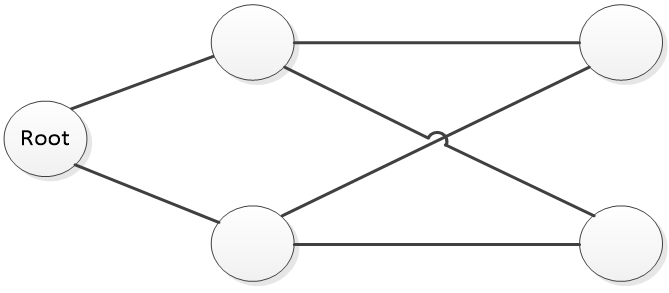
\includegraphics[width=.5\linewidth]{topology}
    \caption{Схема каналов взаимодействия процессов в кластере}
    \label{fig:topology}
\end{figure}


\section{Ход работы}
Текст программы:
\begin{lstlisting}
#include <mpi.h> 
#include <iostream> 
#include <fstream> 
  
#define MESSAGE_LEN 1001 
  
using namespace std; 
  
MPI_Status status; 
char *message; 
int *fullMatrix; 
int *skeletonMatrix; 
  
int index(int i, int j, int n) { 
    return i * n + j; 
} 
  
void init(int n) { 
    ifstream f_in("full.txt"); 
    ifstream s_in("skeleton.txt"); 
    for (int i = 0; i < n; i++) { 
        for (int j = 0; j < n; j++) { 
            f_in >> fullMatrix[index(i, j, n)]; 
            s_in >> skeletonMatrix[index(i, j, n)]; 
        } 
    } 
    f_in.close(); 
    s_in.close(); 
} 
  
void print(int *matrix, int n) { 
    for (int i = 0; i < n; i++) { 
        for (int j = 0; j < n; j++) { 
            cout << matrix[index(i, j, n)] << " "; 
        } 
        cout << endl; 
    } 
} 
  
void master(int size, int rank) { 
    init(size); 
  
    MPI_Barrier(MPI_COMM_WORLD); 
    MPI_Bcast(fullMatrix, size * size, MPI_INT, 0, MPI_COMM_WORLD); 
  
    MPI_Barrier(MPI_COMM_WORLD); 
    MPI_Bcast(skeletonMatrix, size * size, MPI_INT, 0, MPI_COMM_WORLD); 
  
    cout << "Please input message: (max " << (MESSAGE_LEN - 1) / 2 << ")" << endl; 
    message = new char[MESSAGE_LEN]; 
    cin.getline(message, MESSAGE_LEN); 
    cout << endl; 
  
    int sendCount = 0; 
    for (int i = 0; i < size; i++) { 
        if (skeletonMatrix[index(rank, i, size)] == 1) { 
            MPI_Send(message, MESSAGE_LEN, MPI_CHAR, i, 0, MPI_COMM_WORLD); 
            sendCount++; 
        } 
    } 
  
    while (sendCount) { 
        MPI_Recv(NULL, 0, MPI_INT, MPI_ANY_SOURCE, 1, MPI_COMM_WORLD, &status); 
        sendCount--; 
    } 
  
    cout << endl << "Full matrix: " << endl; 
    print(fullMatrix, size); 
    cout << endl << "Skeleton matrix: " << endl; 
    print(skeletonMatrix, size); 
} 
  
void slave(int size, int rank) { 
    MPI_Barrier(MPI_COMM_WORLD); 
    MPI_Bcast(fullMatrix, size * size, MPI_INT, 0, MPI_COMM_WORLD); 
  
    MPI_Barrier(MPI_COMM_WORLD); 
    MPI_Bcast(skeletonMatrix, size * size, MPI_INT, 0, MPI_COMM_WORLD); 
  
    message = new char[MESSAGE_LEN]; 
    MPI_Recv(message, MESSAGE_LEN, MPI_CHAR, MPI_ANY_SOURCE, 0, MPI_COMM_WORLD, &status); 
    cout << "r[" << status.MPI_SOURCE << "] -> r[" << rank << "]: '" << message << "'" << endl; 
  
    int countSends = 0; 
    for (int i = 0; i < size; i++) { 
        if (skeletonMatrix[index(rank, i, size)] == 1) { 
            MPI_Send(message, MESSAGE_LEN, MPI_CHAR, i, 0, MPI_COMM_WORLD); 
            countSends++; 
        } 
    } 
  
    for (; countSends; countSends--) { 
        MPI_Recv(NULL, 0, MPI_INT, MPI_ANY_SOURCE, 1, MPI_COMM_WORLD, NULL); 
    } 
    MPI_Send(NULL, 0, MPI_INT, status.MPI_SOURCE, 1, MPI_COMM_WORLD); 
} 
  
int main(int argc, char **argv) { 
    int size, rank; 
    MPI_Init(&argc, &argv); 
    MPI_Comm_rank(MPI_COMM_WORLD, &rank); 
    MPI_Comm_size(MPI_COMM_WORLD, &size); 
  
    fullMatrix = new int[size * size]; 
    skeletonMatrix = new int[size * size]; 
    !rank ? master(size, rank) : slave(size, rank); 
  
    MPI_Finalize(); 
    return 0; 
}  
\end{lstlisting}

На рисунке \ref{fig:result} представлен результат работы программы:
\begin{figure}[H]
    \centering
    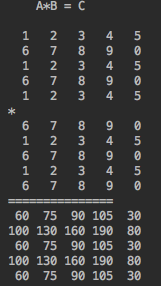
\includegraphics[width=.5\linewidth]{result}
    \caption{Результат работы программы}
    \label{fig:result}
\end{figure}

\section*{Выводы}
В ходе выполнения лабораторной работы были исследованы алгоритмические методы
построения взаимодействия распределено выполняющихся процессов, закреплены
практические навыки построения модели \enquote{зонд-эхо},
\enquote{распределенных семафоров} и \enquote{передача маркера}.
\end{document}